\documentclass[a4paper]{article}
% -------------------------------PACKAGES-------------------------------
\usepackage{amsmath,amsfonts,amssymb}   % for math
\usepackage{indentfirst}    % for indenting first para after section
\usepackage{xcolor}         % for coloured text
\usepackage{colortbl}       % for cell colours
\usepackage{listings}       % for Python text
\usepackage{graphicx}       % for images
\usepackage{hyperref}       % for hyperlinks & internal references
\usepackage[utf8]{inputenc} % for best practice
\setlength{\parskip}{1em}   % length between paras

% Hyper links style
\hypersetup{
    colorlinks=true,
    linkcolor=darkgray,
    filecolor=magenta,      
    urlcolor=cyan,
    pdftitle={Overleaf Example},
    pdfpagemode=FullScreen,
}

% Python-style environment setup
\definecolor{codegreen}{rgb}{0,0.6,0}
\definecolor{codegray}{rgb}{0.5,0.5,0.5}
\definecolor{codepurple}{rgb}{0.58,0,0.82}
\definecolor{backcolour}{rgb}{0.95,0.95,0.92}

\lstdefinestyle{mystyle}{
    backgroundcolor=\color{backcolour},   
    commentstyle=\color{codegreen},
    keywordstyle=\color{magenta},
    numberstyle=\tiny\color{codegray},
    stringstyle=\color{codepurple},
    basicstyle=\ttfamily\footnotesize,
    breakatwhitespace=false,         
    breaklines=true,                 
    captionpos=b,                    
    keepspaces=true,                 
    showspaces=false,                
    showstringspaces=false,
    showtabs=false,                  
    tabsize=2
}
\lstset{style=mystyle}

% Boilerplate
\title{CAR PARK MANAGEMENT SYSTEM \& SIMULATOR REPORT\vspace{-3ex}}
\author{Solo Team - Group 111\\Johnny Madigan} % remove nNumber before uploading to github
\date{\vspace{-3ex}October 2021\vspace{20ex}}

\begin{document}
\maketitle
\begin{center}
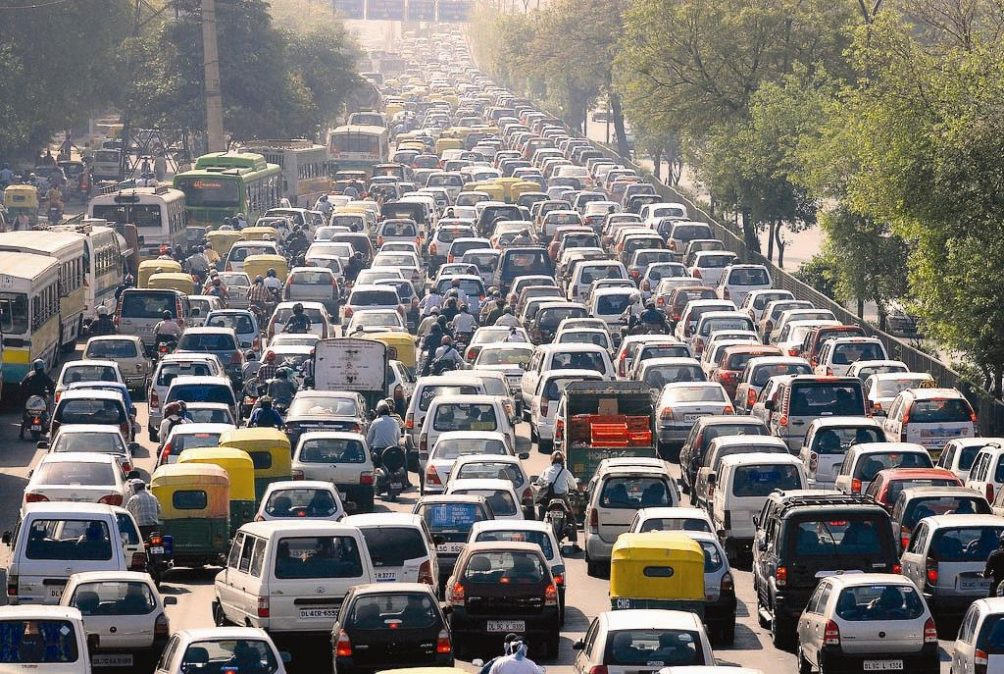
\includegraphics[width=7cm]{report-img/title-pic.jpg}
\end{center}
\newpage
\tableofcontents
\newpage

% ---------------------STATEMENT OF CONTRIBUTION---------------------
\section{Demonstration Video}\label{sec:demo}

\par \href{https://youtu.be/-4QtDzU25com}{YouTube Link}

% ---------------------STATEMENT OF CONTRIBUTION---------------------
\section{Statement of Contribution}\label{sec:contribution}

\begin{tabular}{ |l|l| }
\hline
 \cellcolor{gray!10}\textbf{Johnny Madigan} & Invented, designed, documented, \& demonstrated\\
\hline
\end{tabular}

% ---------------------STATEMENT OF COMPLETENESS---------------------
\section{Statement of Completeness}\label{sec:completeness}

\subsection{General requirements}
\begin{tabular}{|m{24.7em}|l|}
  \hline
  \cellcolor{gray!10} \textbf{Feature\slash Requirement} & \cellcolor{gray!10} \textbf{Status}\\
  \hline
  Configurable no. of entrances/exits/levels 1-5 & \cellcolor{green!40}Implemented\\
  \hline
  Configurable capacity per level & \cellcolor{green!40}Implemented\\
  \hline
  Configurable min/max temperatures & \cellcolor{green!40}Implemented\\
  \hline
  Configurable chance of spawning authorised cars & \cellcolor{green!40}Implemented\\
  \hline
  Configurable duration for running all 3 programs & \cellcolor{green!40}Implemented\\
  \hline
  Configurable slow motion & \cellcolor{green!40}Implemented\\
  \hline
\end{tabular}

\subsection{Simulator Requirements}
\begin{tabular}{|m{24.7em}|l|}
  \hline
  \cellcolor{gray!10} \textbf{Feature\slash Requirement} & \cellcolor{gray!10} \textbf{Status}\\
  \hline
  Simulates movement of vehicles around the car park &\cellcolor{green!40}Implemented\\
  \hline
  Simulates hardware (LPRs, boom gates, signs, alarms, temperature sensors) & \cellcolor{green!40}Implemented\\
  \hline
  Checks bounds of \emph{config.h} as these are user inputs prone to human-error & \cellcolor{green!40}Implemented\\
  \hline
  Creates a dynamic shared memory object &\cellcolor{green!40}Implemented\\
  \hline
  Shared memory’s structure complies with specification &\cellcolor{green!40}Implemented\\
  \hline
  Shared memory is setup for inter-process communication &\cellcolor{green!40}Implemented\\
  \hline
  Avoids busy-waiting where possible & \cellcolor{green!40}Implemented\\
  \hline
  Strict synchronisation using mutex locks/condition variables to avoid race-conditions/deadlocks & \cellcolor{green!40}Implemented\\
  \hline
  Spawn cars every 1-100ms with random license plate& \cellcolor{green!40}Implemented\\
  \hline
  Random license plate has a chance of being authorised & \cellcolor{green!40}Implemented\\
  \hline
  Cars queue outside random entrances & \cellcolor{green!40}Implemented\\
  \hline
  Cars trigger entrance LPR after 2ms & \cellcolor{green!40}Implemented\\
  \hline
  Entrance threads read license plates into LPR and broadcasts Manager for decision-making & \cellcolor{green!40}Implemented\\
  \hline
  Cars read the digital sign and act accordingly & \cellcolor{green!40}Implemented\\
  \hline
  Car leaves simulation if sign displays not authorised (X) & \cellcolor{green!40}Implemented\\
  \hline
\end{tabular}

\begin{tabular}{|m{24.7em}|l|}
  \hline
  Car leaves simulation if sign displays car park is full (F) & \cellcolor{green!40}Implemented\\
  \hline
  Car leaves simulation if sign displays “EVACUATE” & \cellcolor{green!40}Implemented\\
  \hline
  Car enters if assigned a level no. & \cellcolor{green!40}Implemented\\
  \hline
  Sets gates to opened if being raised (10ms) & \cellcolor{green!40}Implemented\\
  \hline
  Sets gates to closed if being lowered (10ms) & \cellcolor{green!40}Implemented\\
  \hline
  Authorised cars that enter are given their own thread so they can move/park independently & \cellcolor{green!40}Implemented\\
  \hline
  Cars take 10ms to drive to their assigned level from the entrance & \cellcolor{green!40}Implemented\\
  \hline
  Cars take 10ms to drive to a random exit after parking & \cellcolor{green!40}Implemented\\
  \hline
  Cars trigger the level LPR when entering/exiting & \cellcolor{green!40}Implemented\\
  \hline
  Cars queue at their random exit & \cellcolor{green!40}Implemented\\
  \hline
  Exit threads read license plates into LPR and broadcasts Manager for billing & \cellcolor{green!40}Implemented\\
  \hline
  Simulates temperature (1-5ms) per level using an algorithm to be as realistic as possible & \cellcolor{green!40}Implemented\\
  \hline
  Ability to simulate a fire after configuring the minimum/maximum temperatures & \cellcolor{green!40}Implemented\\
  \hline
  Fires (rise or spike in temperature) trigger the Fire-Alarm System & \cellcolor{green!40}Implemented\\
  \hline
  Cars park for a random amount of time (100-10000ms) & \cellcolor{green!40}Implemented\\
  \hline
  Unusual behaviour & \cellcolor{red!40}Absent\\
  \hline
\end{tabular}

\subsection{Manager requirements}
\begin{tabular}{|m{24.7em}|l|}
  \hline
  \cellcolor{gray!10} \textbf{Feature\slash Requirement} & \cellcolor{gray!10} \textbf{Status}\\
  \hline
  Automates aspects of running a car park & \cellcolor{green!40}Implemented\\
  \hline
  Checks bounds of \emph{config.h} as these are user inputs prone to human-error & \cellcolor{green!40}Implemented\\
  \hline
  Reads in authorised license plates from \emph{plates.txt} into hash-table & \cellcolor{green!40}Implemented\\
  \hline
  Validates license plate format and length before adding to hash-table & \cellcolor{green!40}Implemented\\
  \hline
  Locates and maps shared memory object to its data space & \cellcolor{green!40}Implemented\\
  \hline
  Communicates with Simulator and Fire-Alarm System via inter-process communication & \cellcolor{green!40}Implemented\\
  \hline
  Monitor status of all LPR sensors & \cellcolor{green!40}Implemented\\
  \hline
  Keeps track of which car is assigned to which level & \cellcolor{green!40}Implemented\\
  \hline
  Keeps track of each level’s current capacity to direct new cars to avaliable spaces & \cellcolor{green!40}Implemented\\
  \hline
  Keeps track of car park’s total capacity (full or not) & \cellcolor{green!40}Implemented\\
  \hline
  Keeps track of total customers for the simulation & \cellcolor{green!40}Implemented\\
  \hline
  Ability to raise gate if closed & \cellcolor{green!40}Implemented\\
  \hline
  Ability to lower gate if opened & \cellcolor{green!40}Implemented\\
  \hline
  Keeps gates opened for 20ms before lowering & \cellcolor{green!40}Implemented\\
  \hline
  Controls sign display & \cellcolor{green!40}Implemented\\
  \hline
  Updates sign display to ‘F’ if car park full & \cellcolor{green!40}Implemented\\
  \hline
\end{tabular}

\begin{tabular}{|m{24.7em}|l|}
  \hline
  Updates sign display to ‘X’ if car is not authorised & \cellcolor{green!40}Implemented\\
  \hline
  Updates sign display to a level no. assigned to authorised cars & \cellcolor{green!40}Implemented\\
  \hline
  Keeps track of how long each car's journey is (time entered-time leaving) & \cellcolor{green!40}Implemented\\
  \hline
  Bills cars at 5 cents per millisecond & \cellcolor{green!40}Implemented\\
  \hline
  Appends billing information to \emph{billing.txt} & \cellcolor{green!40}Implemented\\
  \hline
  Monitors status each level’s alarm and acts accordingly & \cellcolor{green!40}Implemented\\
  \hline
  Displays status of all hardware (LPRs, boom gates, signs, alarms, and temperature sensors) & \cellcolor{green!40}Implemented\\
  \hline
  Displays status of each level’s current capacity and total capacity & \cellcolor{green!40}Implemented\\
  \hline
  Displays total customers so far & \cellcolor{green!40}Implemented\\
  \hline
  Displays total revenue earned so far(\$\$\$) & \cellcolor{green!40}Implemented\\
  \hline
  Updates this display frequently (every 50ms) & \cellcolor{green!40}Implemented\\
  \hline
\end{tabular}

\subsection{Fire-Alarm System requirements}
\begin{tabular}{|m{24.7em}|l|}
  \hline
  \cellcolor{gray!10} \textbf{Feature\slash Requirement} & \cellcolor{gray!10} \textbf{Status}\\
  \hline
  Detects potential fires using 2 algorithms (rise/spike in temperature) & \cellcolor{green!40}Implemented\\
  \hline
  Complies with safety-critical guidelines where possible (\emph{MISRA C/The Power of 10}) & \cellcolor{green!40}Implemented\\
  \hline
  Checks bounds of \emph{config.h} as these are user inputs prone to human-error & \cellcolor{green!40}Implemented\\
  \hline
  Locates and maps shared memory object to its data space & \cellcolor{green!40}Implemented\\
  \hline
  Communicates with Simulator and Manager via inter-process communication & \cellcolor{green!40}Implemented\\
  \hline
  Monitors and collects each level's current temperature every 2ms & \cellcolor{green!40}Implemented\\
  \hline
  Keeps track of each level's 5 most recent temperatures & \cellcolor{green!40}Implemented\\
  \hline
  When 5 temps are collected, the median is the next smoothed temp & \cellcolor{green!40}Implemented\\
  \hline
  Keeps track of each level's 30 most recently smoothed temps & \cellcolor{green!40}Implemented\\
  \hline
  Uses an algorithm for detecting if 90\% or more smoothed temps are 58+ degrees & \cellcolor{green!40}Implemented\\
  \hline
  Uses a 2nd algorithm for detecting if the most recent smoothed temp is 8+ degrees hotter than the 30th most recent smoothed temp & \cellcolor{green!40}Implemented\\
  \hline
  Activates all alarms in the event of a fire & \cellcolor{green!40}Implemented\\
  \hline
  Starts raising all boom gates in the event of a fire & \cellcolor{green!40}Implemented\\
  \hline
  Cycles through each letter of “EVACUATE” and displays it on all signs (every 20ms) & \cellcolor{green!40}Implemented\\
  \hline
\end{tabular}

% ---------------------USAGE---------------------
\newpage
\section{Usage}

\noindent The project structure includes 3 source folders, one for each program. In the main directory, \emph{plates.txt} contains the list of authorised license plates (which you can update), and a configuration file called \emph{config.h}. \emph{plates.txt} MUST stay in the same directory as the executables, as the Simulator and Manager read this file to get the authorised license plates.

\noindent 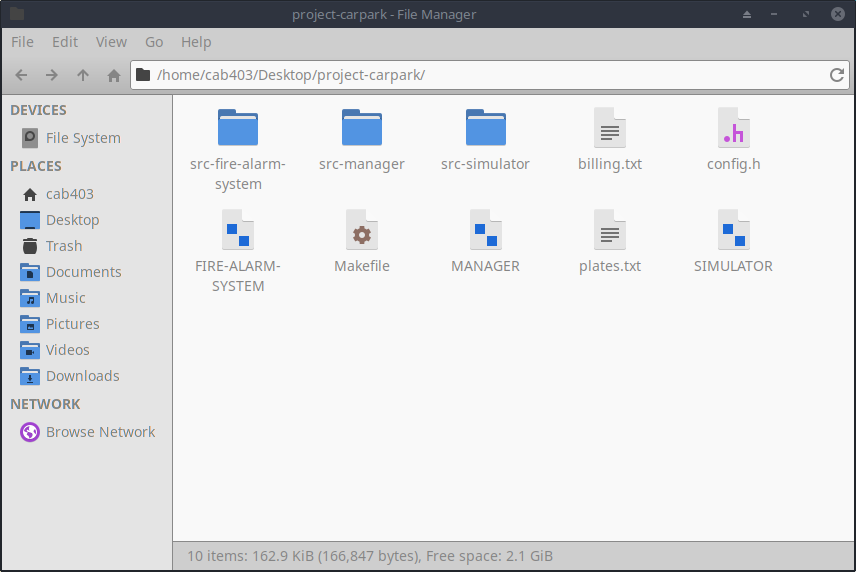
\includegraphics[width=12.12cm]{report-img/project-structure.png}

\noindent \emph{config.h} allows you to customise the simulation in the following ways:
\begin{itemize}
  \item Number of entrances, exits, and levels
  \item Parking capacity for each level
  \item Chance of spawning an authorised car
  \item Duration all 3 programs will run for
  \item Minimum and maximum temperatures
  \item Slow motion
\end{itemize}

\noindent Each source folder has its own Makefile, so you can clean and rebuild each program individually. There is a central Makefile in the main directory, which can clean and rebuild all 3 Makefiles at once. After building, 3 executable will be created in the main directory. When running the programs, make sure to run the Simulator first, as it's responsible for creating the shared memory object that the Simulator, Manager, and Fire-Alarm System will use to communicate between each-other. Please open 3 terminal windows and run each program in its own window. Please navigate into the main directory to run the following:

\noindent To clean:
\begin{lstlisting}[language=bash]
  $ make clean
\end{lstlisting}

\noindent To build:
\begin{lstlisting}[language=bash]
  $ make
\end{lstlisting}

\noindent To run the Simulator:
\begin{lstlisting}[language=bash]
  $ ./SIMULATOR
\end{lstlisting}

\noindent To run the Manager:
\begin{lstlisting}[language=bash]
  $ ./MANAGER
\end{lstlisting}

\noindent To run the Fire-Alarm System:
\begin{lstlisting}[language=bash]
  $ ./FIRE-ALARM-SYSTEM
\end{lstlisting}


\noindent After the programs finish, there will be a new file called \emph{billing.txt} showing how much each customer was billed during the simulation.

% ---------------------FIRE ALARM ASSESSMENT---------------------
\section{Assessment of the supplied Fire Alarm system}

% ------NASA'S THE POWER OF 10 SUBSECTION------
\subsection{NASA’s \emph{The Power of 10} Violations}

% violation
\par \noindent \textbf{RULE 1 VIOLATION\\“Avoid complex flow constructs, such as goto and recursion”} \\[1\baselineskip]
The system does not avoid complex flow constructs such as \emph{goto} and recursion. A \emph{goto} statement is found in Main and the \emph{deletenodes} function is recursive. \\[1\baselineskip]
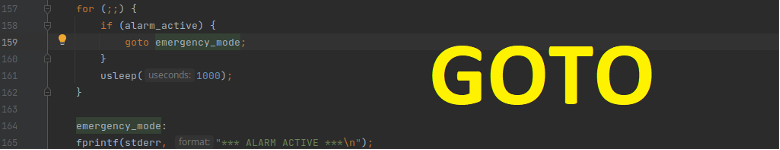
\includegraphics[width=12.12cm]{report-img/nasa-rule-1-violation.png}
\\

\includegraphics[width=12.12cm]{report-img/nasa-rule-1-violation-2.png}

% violation
\newpage
\par \noindent \textbf{RULE 2 VIOLATION\\“All loops must have fixed bounds. This prevents runaway code”} \\[1\baselineskip]
The system contains loops with no fixed bounds, a.k.a. runaway code. These infinite loops are found in Main (causing unreachable code), the \emph{tempmonitor} function (thread will never return), and the \emph{openboomgate} function (thread will never return). \\[1\baselineskip]
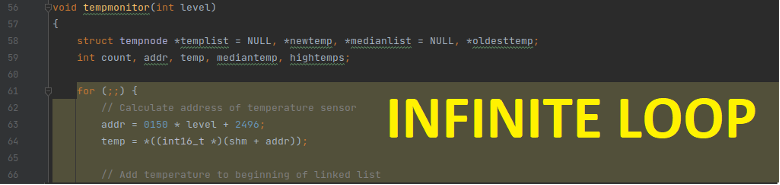
\includegraphics[width=12.12cm]{report-img/nasa-rule-2-violation.png}
\\
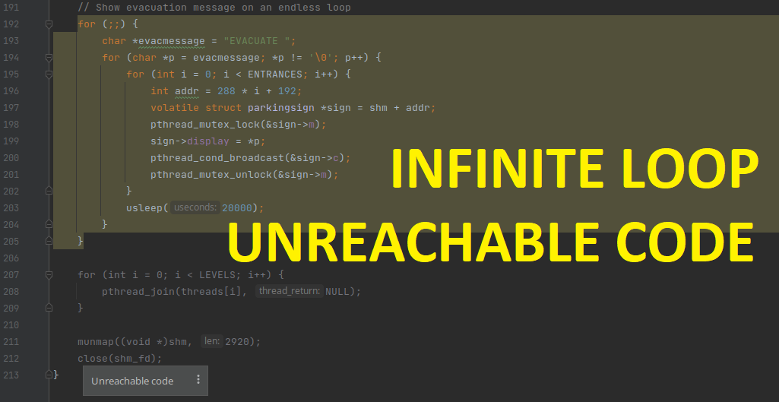
\includegraphics[width=12.12cm]{report-img/nasa-rule-2-violation-2.png}
\\

\includegraphics[width=12.12cm]{report-img/nasa-rule-2-violation-3.png}

% violation
\newpage
\par \noindent \textbf{RULE 3 VIOLATION\\“Avoid heap memory allocation”} \\[1\baselineskip]
The system fails to avoid heap memory allocation (5 times) using the \emph{malloc} function. \\[1\baselineskip]
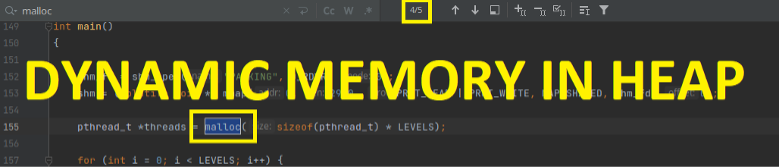
\includegraphics[width=12.12cm]{report-img/nasa-rule-3-violation.png}

% violation
\par \noindent \textbf{RULE 4 VIOLATION\\ “Restrict functions to a single printed page”} \\[1\baselineskip]
The system fails to restrict functions to a single printed page (avoid extremely long/multi-purposed/complex functions). The \emph{tempmonitor} function spans 73 lines. \\[1\baselineskip]

\includegraphics[width=12.12cm]{report-img/nasa-rule-4-violation.png}

% violation
\par \noindent \textbf{RULE 5 VIOLATION\\ “Use a minimum of two runtime assertions per function”} \\[1\baselineskip]
The system fails to use at least 2 runtime assertions. For example, the system should have checked if \emph{shm\_open} and \emph{mmap} worked (not NULL).

% violation
\par \noindent \textbf{RULE 6 VIOLATION\\ “Restrict the scope of data to the smallest possible”} \\[1\baselineskip]
The system fails to restrict scope of data to the smallest possible as there are global variables that do not need to be global. Integer variable \emph{shm\_fd} is only used in \emph{Main} but is declared globally, and volatile void pointer \emph{shm} is also declared globally and defined in main but used only once in another function (\emph{tempmonitor}) and therefore should be passed as an argument to minimise scope. \\[1\baselineskip]
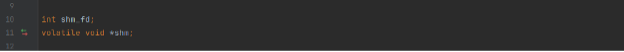
\includegraphics[width=12.12cm]{report-img/nasa-rule-6-violation.png}

% violation
\newpage
\par \noindent \textbf{RULE 10 VIOLATION\\ “Compile with all possible warnings active; all warnings should then be addressed before release of the software”} \\[1\baselineskip]
The system has left a large number of warnings unaddressed when compiled with flags \emph{-Wall -Wextra -pedantic -g}. \\[1\baselineskip]
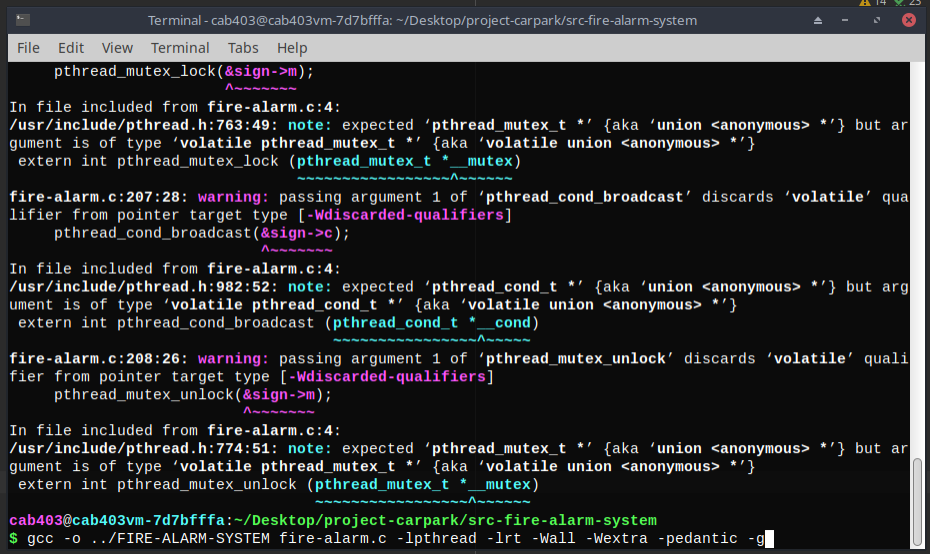
\includegraphics[width=12.12cm]{report-img/nasa-rule-10-violation.png}

% ------MISRA C 2012------
\subsection{\emph{MISRA C:2012} Violations}

% violation
\par \noindent \textbf{Directive 1.1} \\[1\baselineskip]
Although the system contains comments indicating some sections of code, the system fails to document the behaviour of the file itself and functions within (brief, parameters, return values, etc.). \\[1\baselineskip]
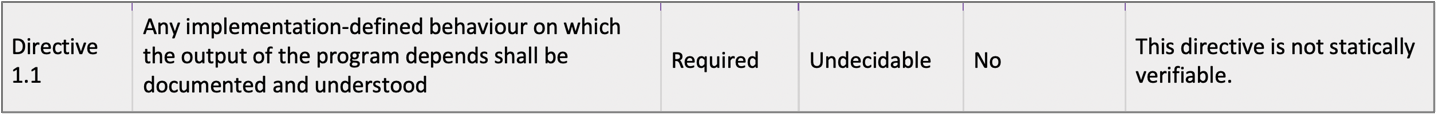
\includegraphics[width=12.12cm]{report-img/misra-c-1.png}

% violation
\par \noindent \textbf{Directive 2.1} \\[1\baselineskip]
Likewise in \emph{The Power of 10} evaluation, the supplied system left a large number of warnings unaddressed when compiling with flags \emph{-Wall -Wextra -pedantic -g}. \\[1\baselineskip]
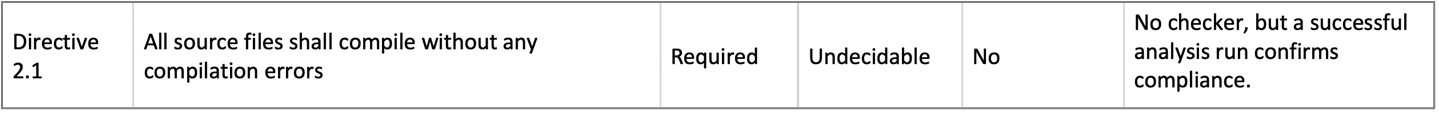
\includegraphics[width=12.12cm]{report-img/misra-c-2.png}

% violation
\newpage
\par \noindent \textbf{Directive 4.12} \\[1\baselineskip]
Likewise in \emph{The Power of 10} evaluation, the system uses the \emph{malloc} function to allocate dynamic memory to the heap 5 times. Furthermore, there was no code following these \emph{malloc} calls to handle failure (when \emph{malloc} returns NULL) nor was the \emph{free} function used to deallocate the heap memory. \\[1\baselineskip]
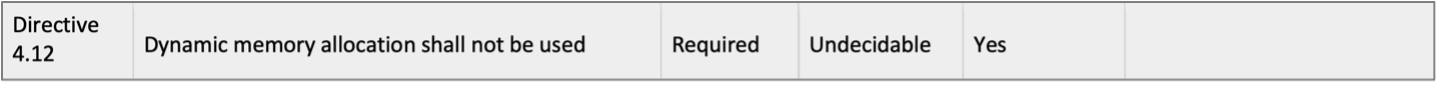
\includegraphics[width=12.12cm]{report-img/misra-c-3.png}

% violation
\par \noindent \textbf{Rule 2.1} \\[1\baselineskip]
An infinite loop near the end of \emph{Main} prevents the system from cleaning up (\emph{munmap} and \emph{shm\_close}) and returning an exit value (although no return value currently implemented). \\[1\baselineskip]

\includegraphics[width=12.12cm]{report-img/misra-c-4.png}

% violation
\par \noindent \textbf{Rule 15.1} \\[1\baselineskip]
The system’s \emph{Main} function uses a \emph{goto} statement to break out of a loop. \\[1\baselineskip]

\includegraphics[width=12.12cm]{report-img/misra-c-5.png}

% violation
\par \noindent \textbf{Rule 15.5} \\[1\baselineskip]
The system’s \emph{deletenodes} function has 2 points of exit. \\[1\baselineskip]

\includegraphics[width=12.12cm]{report-img/misra-c-6.png}

% violation
\par \noindent \textbf{Rule 17.2} \\[1\baselineskip]
The system’s \emph{deletenodes} function is recursive. \\[1\baselineskip]
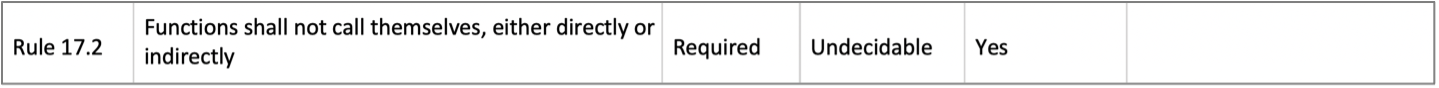
\includegraphics[width=12.12cm]{report-img/misra-c-7.png}

% violation
\par \noindent \textbf{Rule 17.8} \\[1\baselineskip]
The system’s \emph{deletenodes} function modifies a linked-list of temperatures (as it deletes members in the given list). \\[1\baselineskip]

\includegraphics[width=12.12cm]{report-img/misra-c-8.png}

% violation
\newpage
\par \noindent \textbf{Rule 18.4} \\[1\baselineskip]
The system accesses segments of the shared memory object using pointer arithmetic (\emph{shm} + \emph{addr}). \\[1\baselineskip]
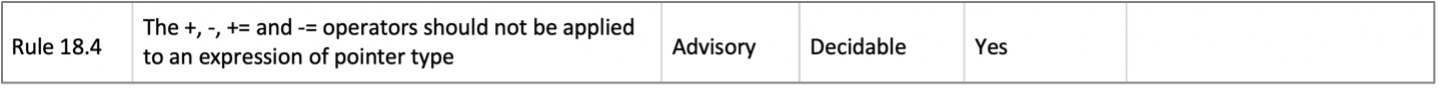
\includegraphics[width=12.12cm]{report-img/misra-c-9.png}

% violation
\par \noindent \textbf{Rule 21.3} \\[1\baselineskip]
Likewise in \emph{The Power of 10} evaluation, the system uses the \emph{malloc} function to allocate dynamic memory to the heap 5 times. Furthermore, there was no code following these \emph{malloc} calls to handle failure (when \emph{malloc} returns \emph{NULL}) nor was the free function used to de-allocate the heap memory. \\[1\baselineskip]
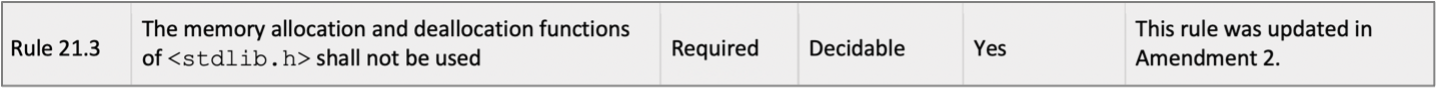
\includegraphics[width=12.12cm]{report-img/misra-c-10.png}

% violation
\par \noindent \textbf{Rule 21.6} \\[1\baselineskip]
The \emph{fprintf} function is used in \emph{Main} to print \emph{“*** ALARM ACTIVE ***”} in standard error message format. \\[1\baselineskip]
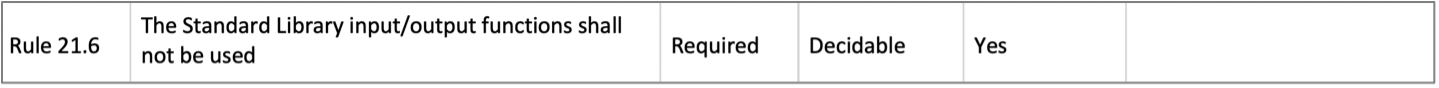
\includegraphics[width=12.12cm]{report-img/misra-c-11.png}

% violation
\par \noindent \textbf{Rule 21.9} \\[1\baselineskip]
The \emph{qsort} function is used to sort temperatures in ascending order to get the median (in the \emph{tempmonitor} function). \\[1\baselineskip]
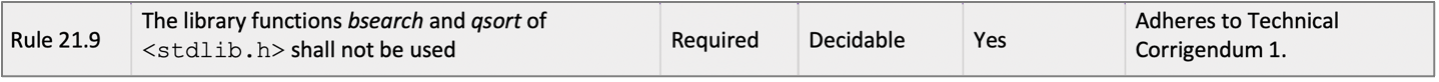
\includegraphics[width=12.12cm]{report-img/misra-c-12.png}

% violation
\par \noindent \textbf{Rule 21.10} \\[1\baselineskip]
Although unused, the system includes the standard \emph{time.h} library. \\[1\baselineskip]
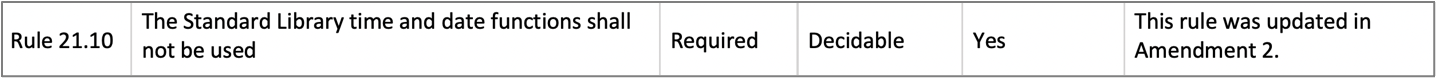
\includegraphics[width=12.12cm]{report-img/misra-c-13.png}

% ------ADDITIONAL PROBLEMS------
\newpage
\subsection{Additional Problems}

% problem
\par \noindent The system’s \emph{Main} function does not have a return value while promising a return value of type integer. \\[1\baselineskip]
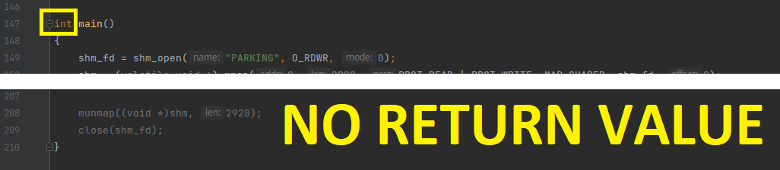
\includegraphics[width=12.12cm]{report-img/other-problem-1.png}

% problem
\par \noindent The system does not meet the requirement of waiting 2 milliseconds before collecting temperatures. \\[1\baselineskip]
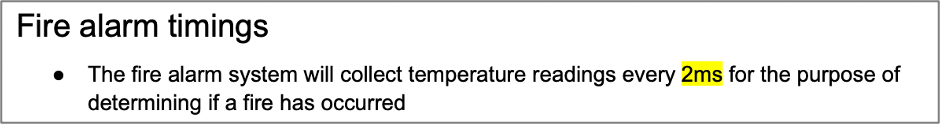
\includegraphics[width=12.12cm]{report-img/other-problem-2.png}

% problem
\par \noindent The system has partially hard-coded the address for accessing exit’s boom gates. \emph{Main} assumes all exit’s boom gates will always be at an offset of 1536 bytes, which is 5 entrances. As there could be anywhere between 1 to 5 entrances inclusive, the system will break immediately. \\[1\baselineskip]
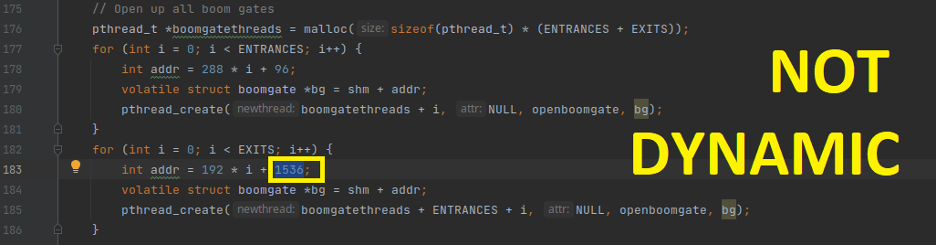
\includegraphics[width=12.12cm]{report-img/other-problem-3.png}

% problem
\par \noindent The system declares 2 unused global variables, a \emph{pthread} mutex lock and \emph{pthread} condition variable for the global alarm indicator. \\[1\baselineskip]
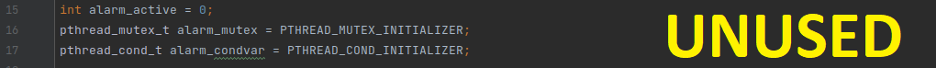
\includegraphics[width=12.12cm]{report-img/other-problem-4.png}

% ------SOLUTION METHOD------
\subsection{Solution method}

\par The approach I used to address the issues highlighted above, was to rewrite the whole program from scratch. This not only allowed me evaluate every decision I was making from a safety-critical POV, but also improve the logic and flow of data.

\newpage
\par I wanted this new implementation to be uniform with the \emph{Simulator} and \emph{Manager}, so it would be easy to read and understand how all 3 programs work together. This meant updating how the system would find and map the shared memory object to its data-space. How the system would locate segments of the shared memory (3 formulas for locating entrances/exits/levels then accessing their hardware via arrow pointer notation). How thread cycles flow (no infinite loops, all threads return when the \emph{end\_simulation} flag is set to true). How thread safety is ensured with mutex locks, condition variables, and the \emph{volatile} and \emph{\_Atomic} keywords. How the program is split into multiple source and header files for modularity/simplicity. And finally, how all bounds are checked/handled, especially \emph{config.h} bounds as these are prone to human error.

\par The 2 key parts of the system that needed to be compliant with safety-critical standards was fixing the recursive linked-list function and replacing the \emph{qsort} function. Rather than deleting linked-list (temperature) nodes recursively, the new implementation simply traverses the entire linked-list and after a certain count, the rest of the nodes will be deleted. The \emph{qsort} function has been replaced with a bubble-sort function that sorts an array in ascending order before returning the median.

% ------CURRENT CONCERNS METHOD------
\subsection{Current safety-critical concerns \& mitigations}

\par When rewriting the fire-alarm system, 3 \emph{MISRA C} guidelines, unfortunately, could not be followed completely. First was no dynamic memory allocation (directive 4.12), second was the use of the standard \emph{time.h} library (rule 21.10), and thirdly was the use of pointer arithmetic (rule 18.4). These violations were mitigated where possible.

\par Regarding dynamic memory, the need to constantly update to hold only the 5 most recent raw temperatures/30 most recently smoothed temperatures, is extremely tedious without the use of dynamic memory. Using a linked-list and its associated operations, greatly reduces code-complexity and overhead. However, as nodes are struct pointers, they must be malloced to have sufficient memory to hold the temperature and a pointer to the next node. This violation has been minimised by limiting the use of the \emph{malloc} function and ensuring that all dynamic memory is released using \emph{free}.

\par The \emph{Simulator} and \emph{Manager} use a custom function for precision when sleeping for milliseconds. However, this requires the \emph{time.h} library for the \emph{timespec} type and \emph{nanosleep} function. Due to sensitive timing being a crucial part of the project, the custom function is still needed here, but isolated in one source/header file.

\par Given the address of the first byte of the shared memory object, pointer arithmetic is necessary to locate items within.

% ------DIAGRAMS------
\section{Diagrams}
\noindent
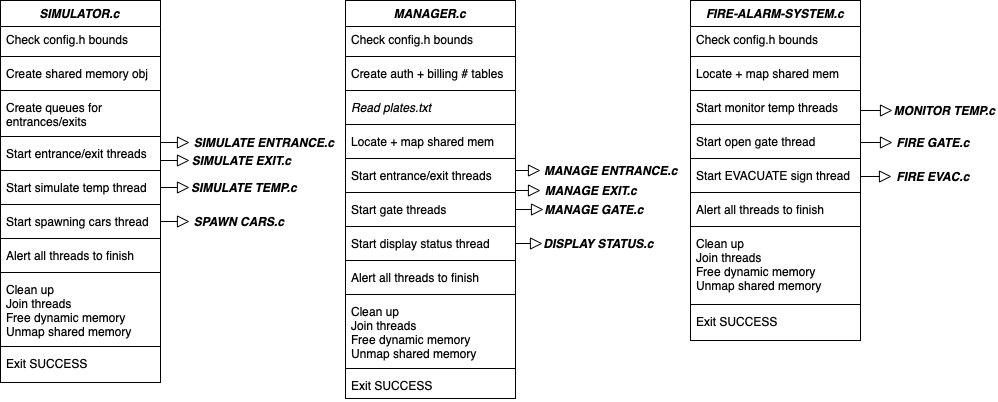
\includegraphics[width=12.12cm]{report-img/diagram-mains.png}\\[5\baselineskip]
\noindent
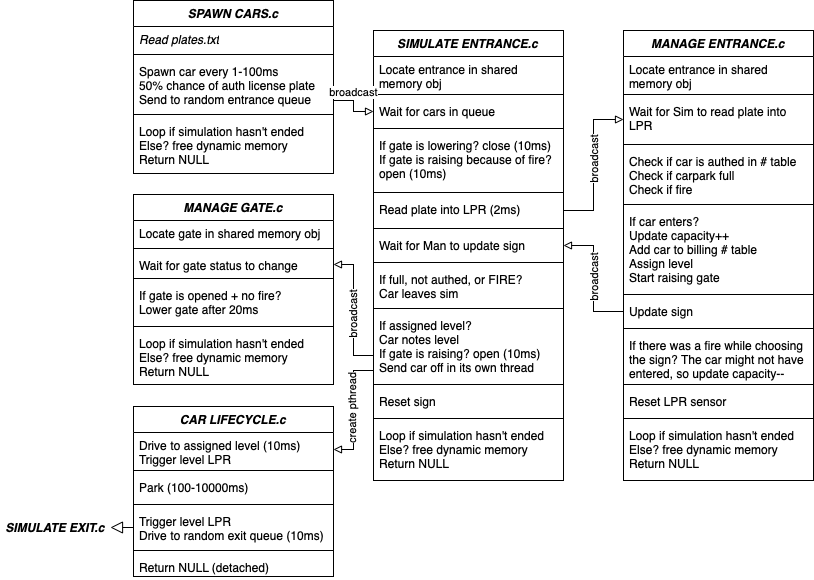
\includegraphics[width=12.12cm]{report-img/diagram-entrance-flow.png}

\newpage
\noindent
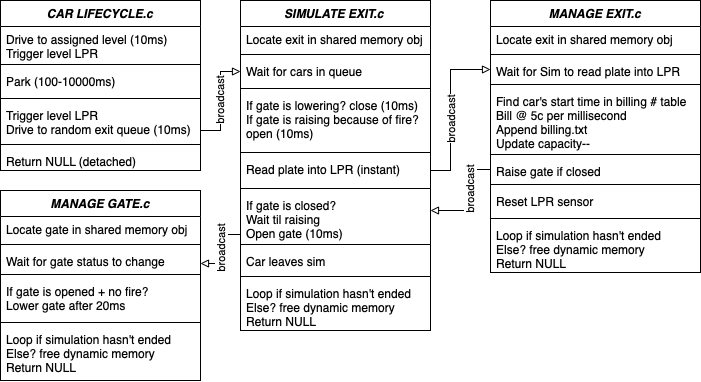
\includegraphics[width=12.12cm]{report-img/diagram-exit-flow.png}\\[5\baselineskip]
\noindent
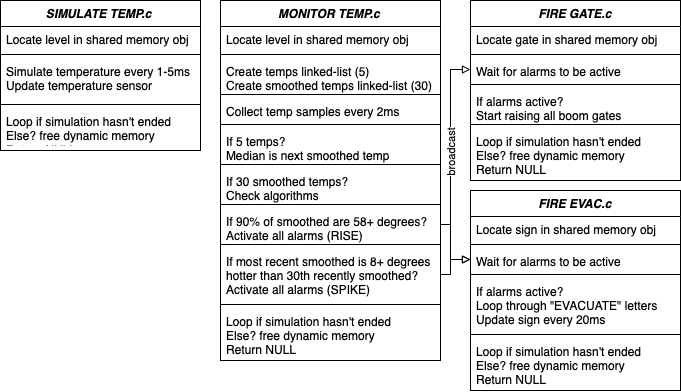
\includegraphics[width=12.12cm]{report-img/diagram-fire-alarm-flow.png}

% ---------------------REFERENCES---------------------
% Some sample references from an old report for an example:

%\section{References}
%\par Garoni, T., Peaker, G., Zongzheng, Z. (2020). \emph{How hard is it to scramble Rubik's Cube?}. Retrieved from\\ \url{https://phys.org/news/2020-01-hard-scramble-rubik-cube.html}

%\par Pocket Cube. (n.d.). \emph{God's Number - looking for the optimal Rubik's Cube solution}. Retrieved from\\ \url{https://ruwix.com/the-rubiks-cube/gods-number/}

%\par Tripi, A. (2017). \emph{Cayley Graphs of Groups and Their Applications}. MSU Graduate Theses. 3133. Retrieved from\\ \url{https://bearworks.missouristate.edu/theses/3133}

\end{document}
